\chapter{Dodatek B}

Niniejszy dodatek zawiera zdjęcia elementów wykonanych w trakcie realizacji projektu.

\begin{figure}[h]
    \centering
    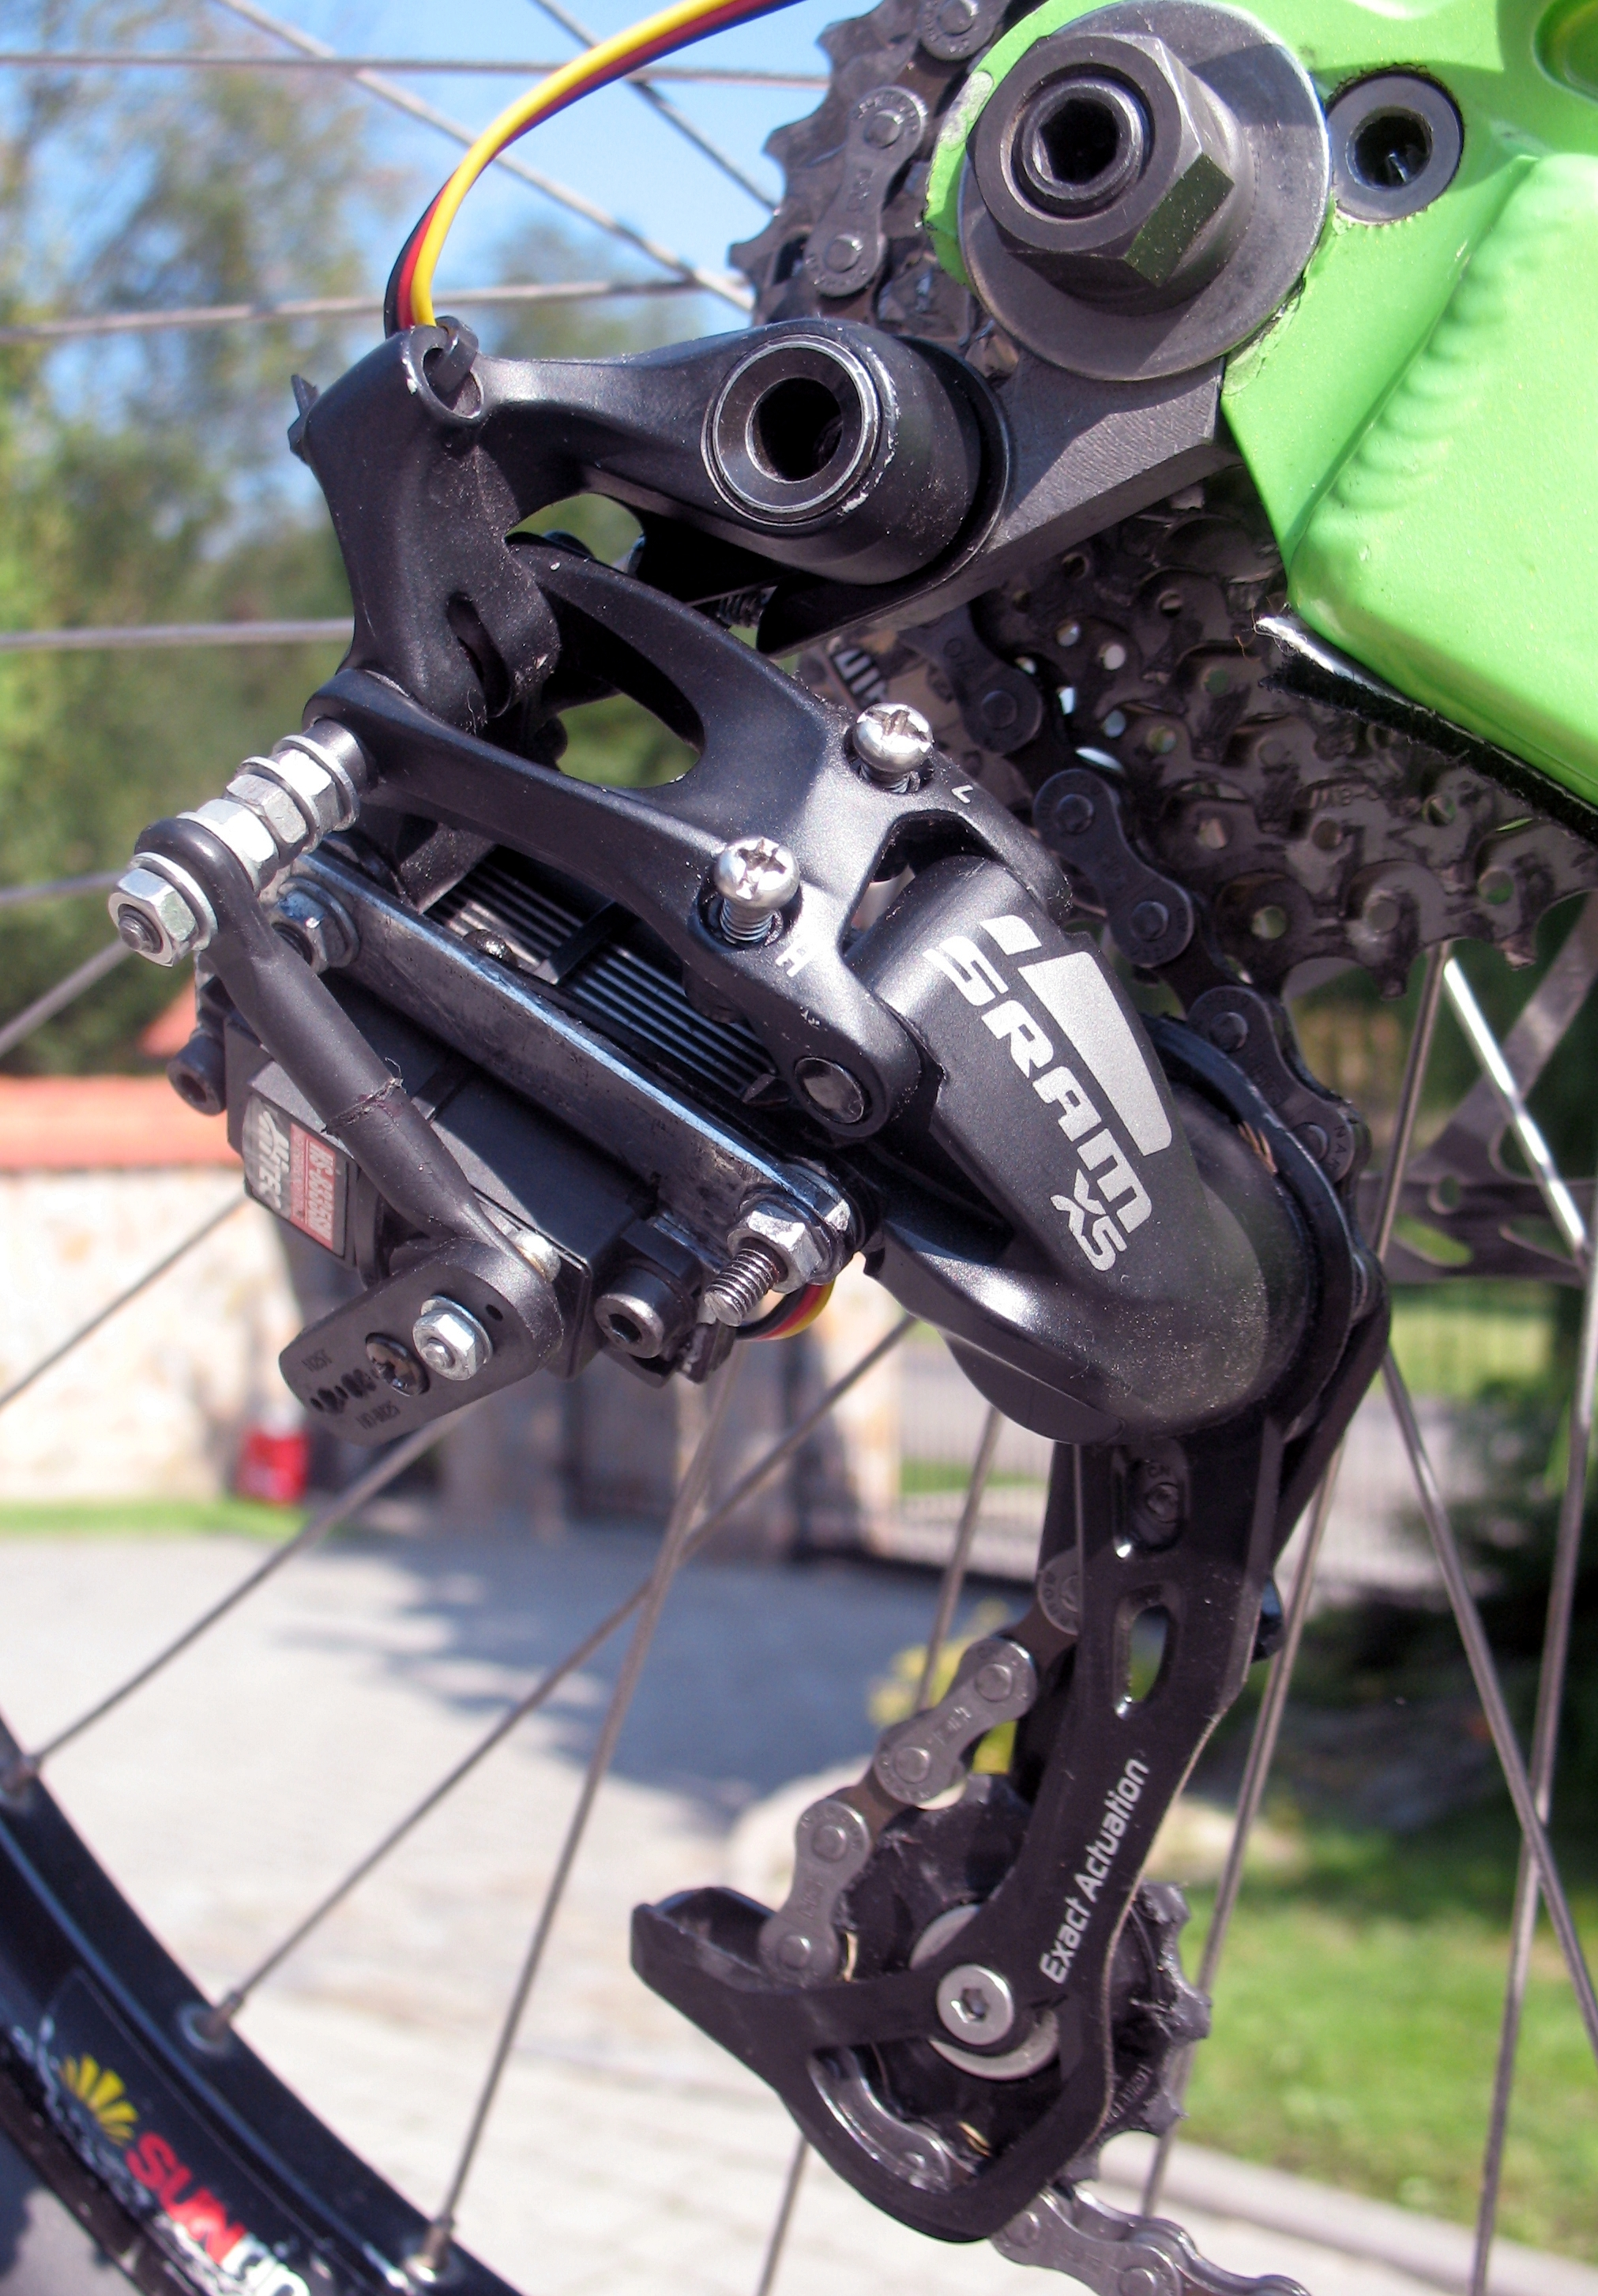
\includegraphics[scale=0.08]{przerzutkaRower.jpg}
    \caption{Przerzutka SRAM X5 wraz z zamontowanym serwomechanizmem.}
    \label{fig:Rower}
\end{figure}


\begin{figure}[h]
\centering
\begin{subfigure}{.4\textwidth}
  \centering
  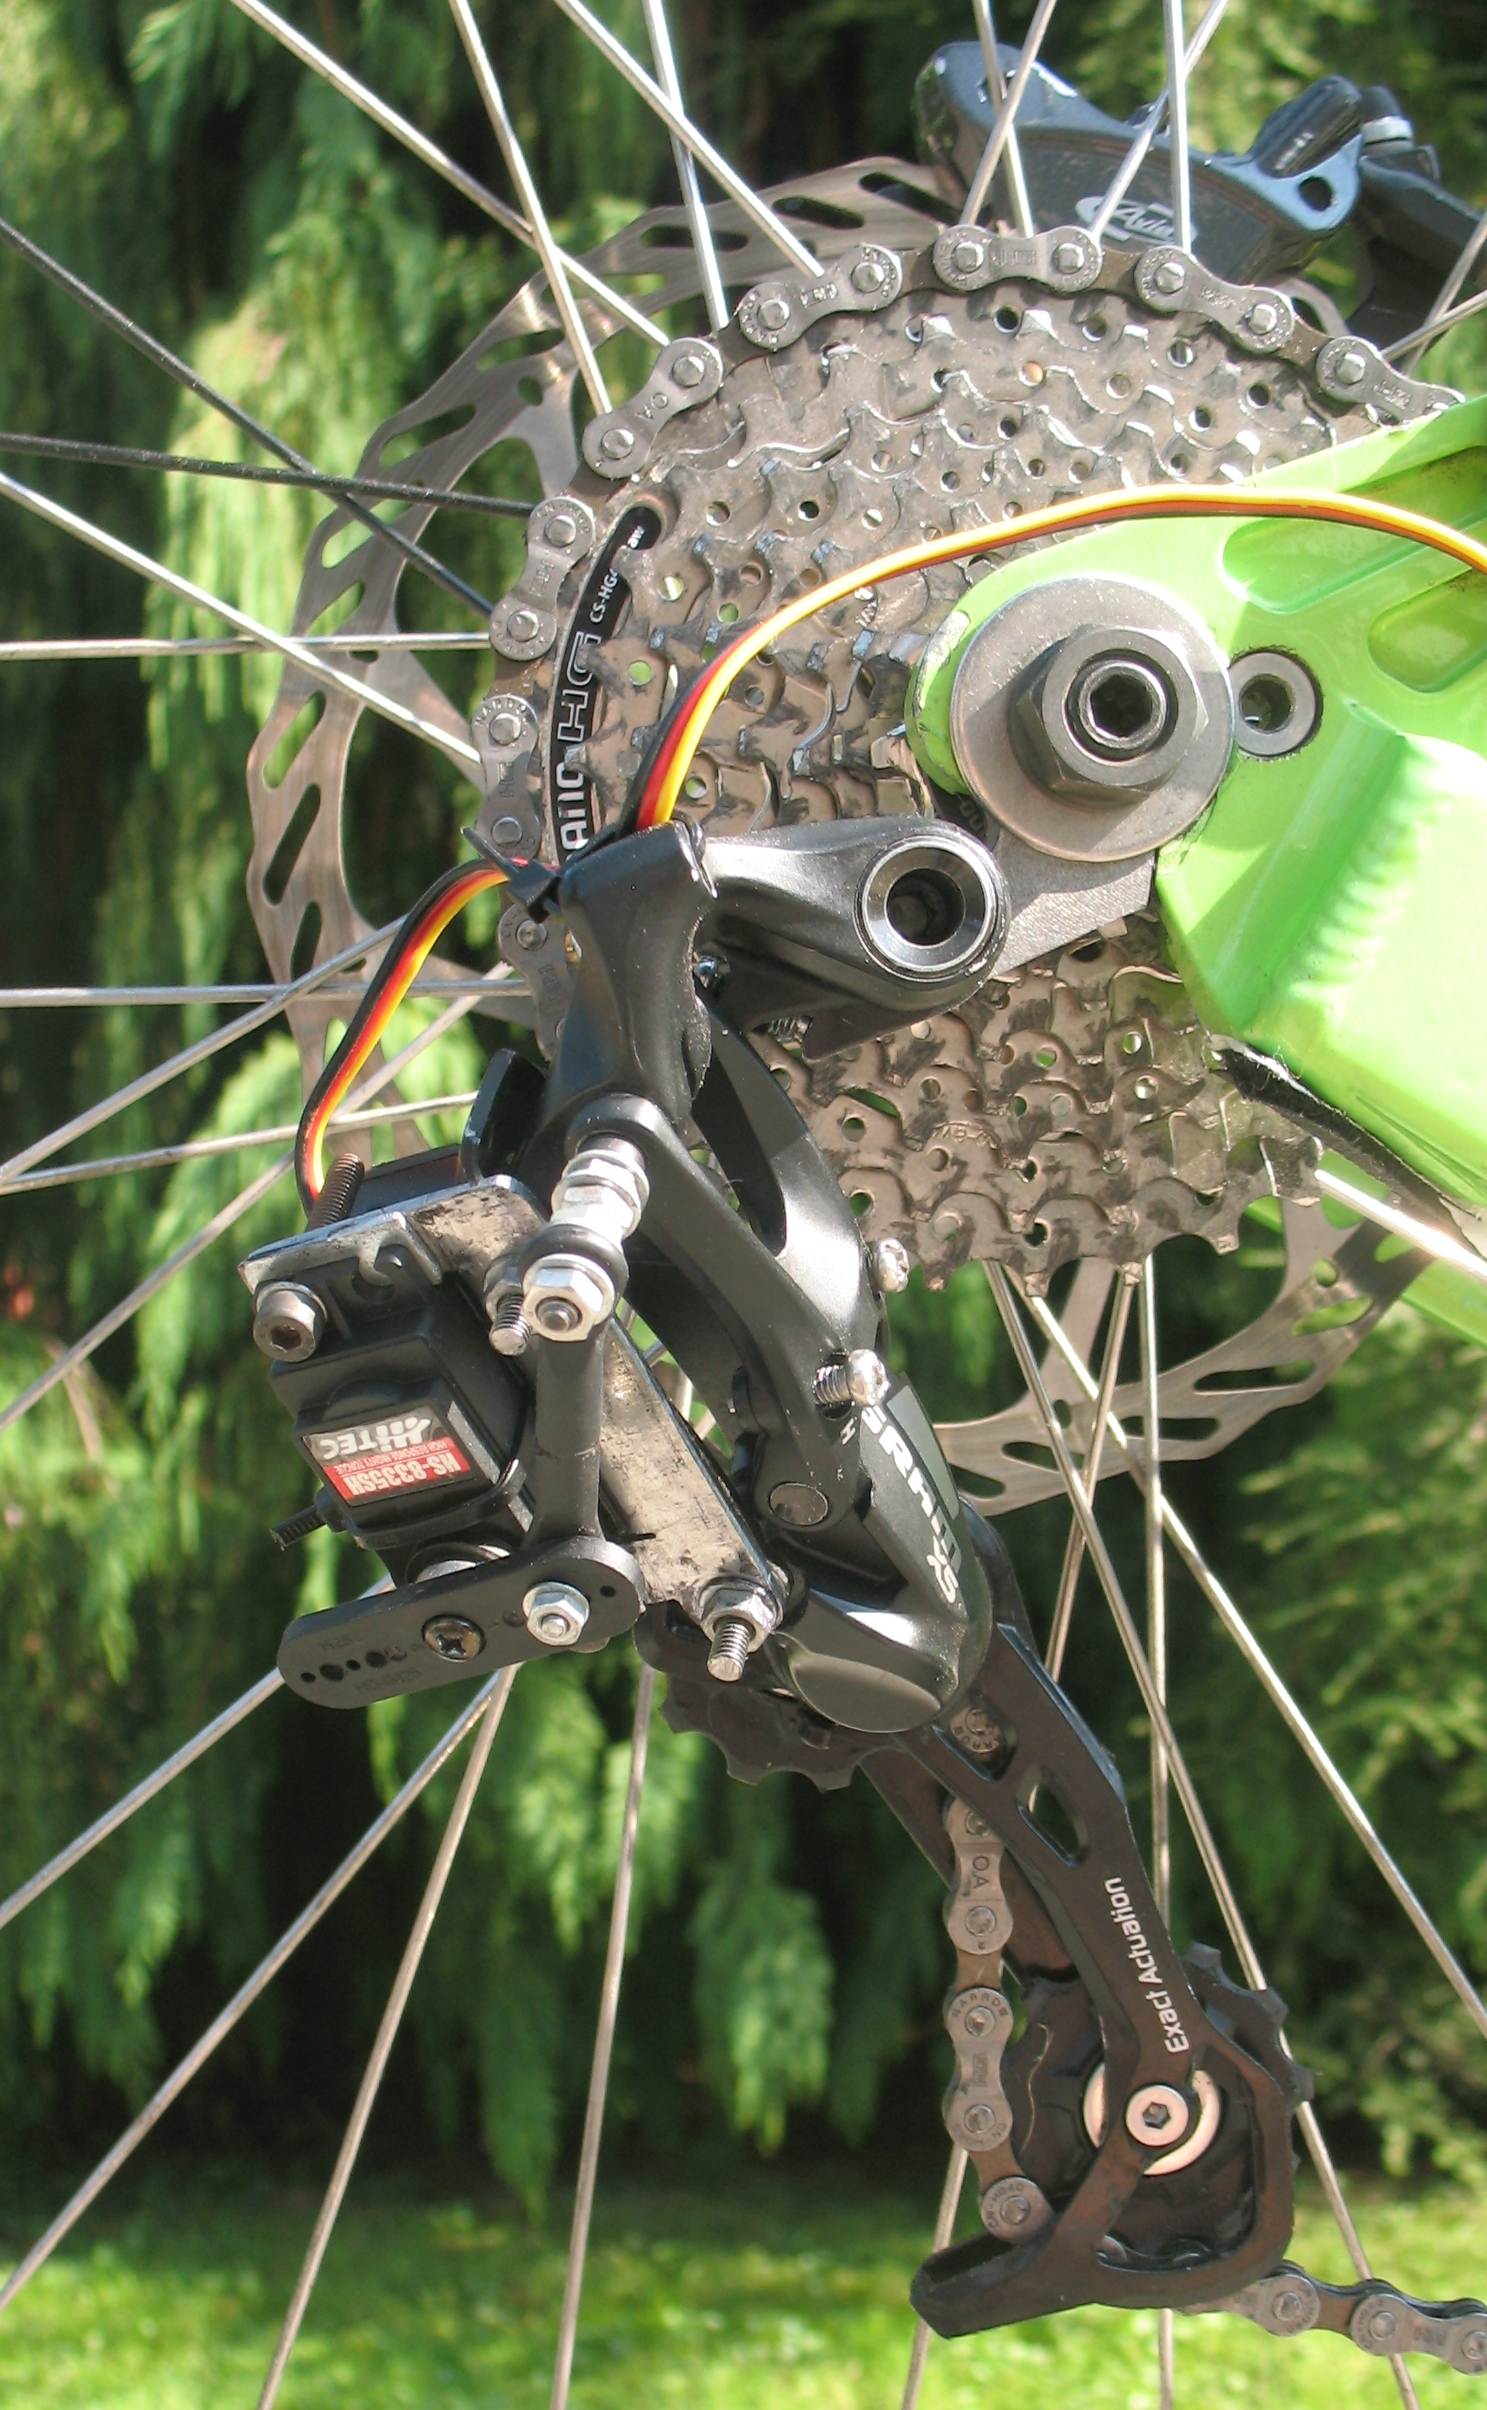
\includegraphics[scale=0.07]{przerzutka1bieg.jpg}
  \caption{Przerzutka w pozycji biegu nr 1}

\end{subfigure}
\begin{subfigure}{.4\textwidth}
  \centering
  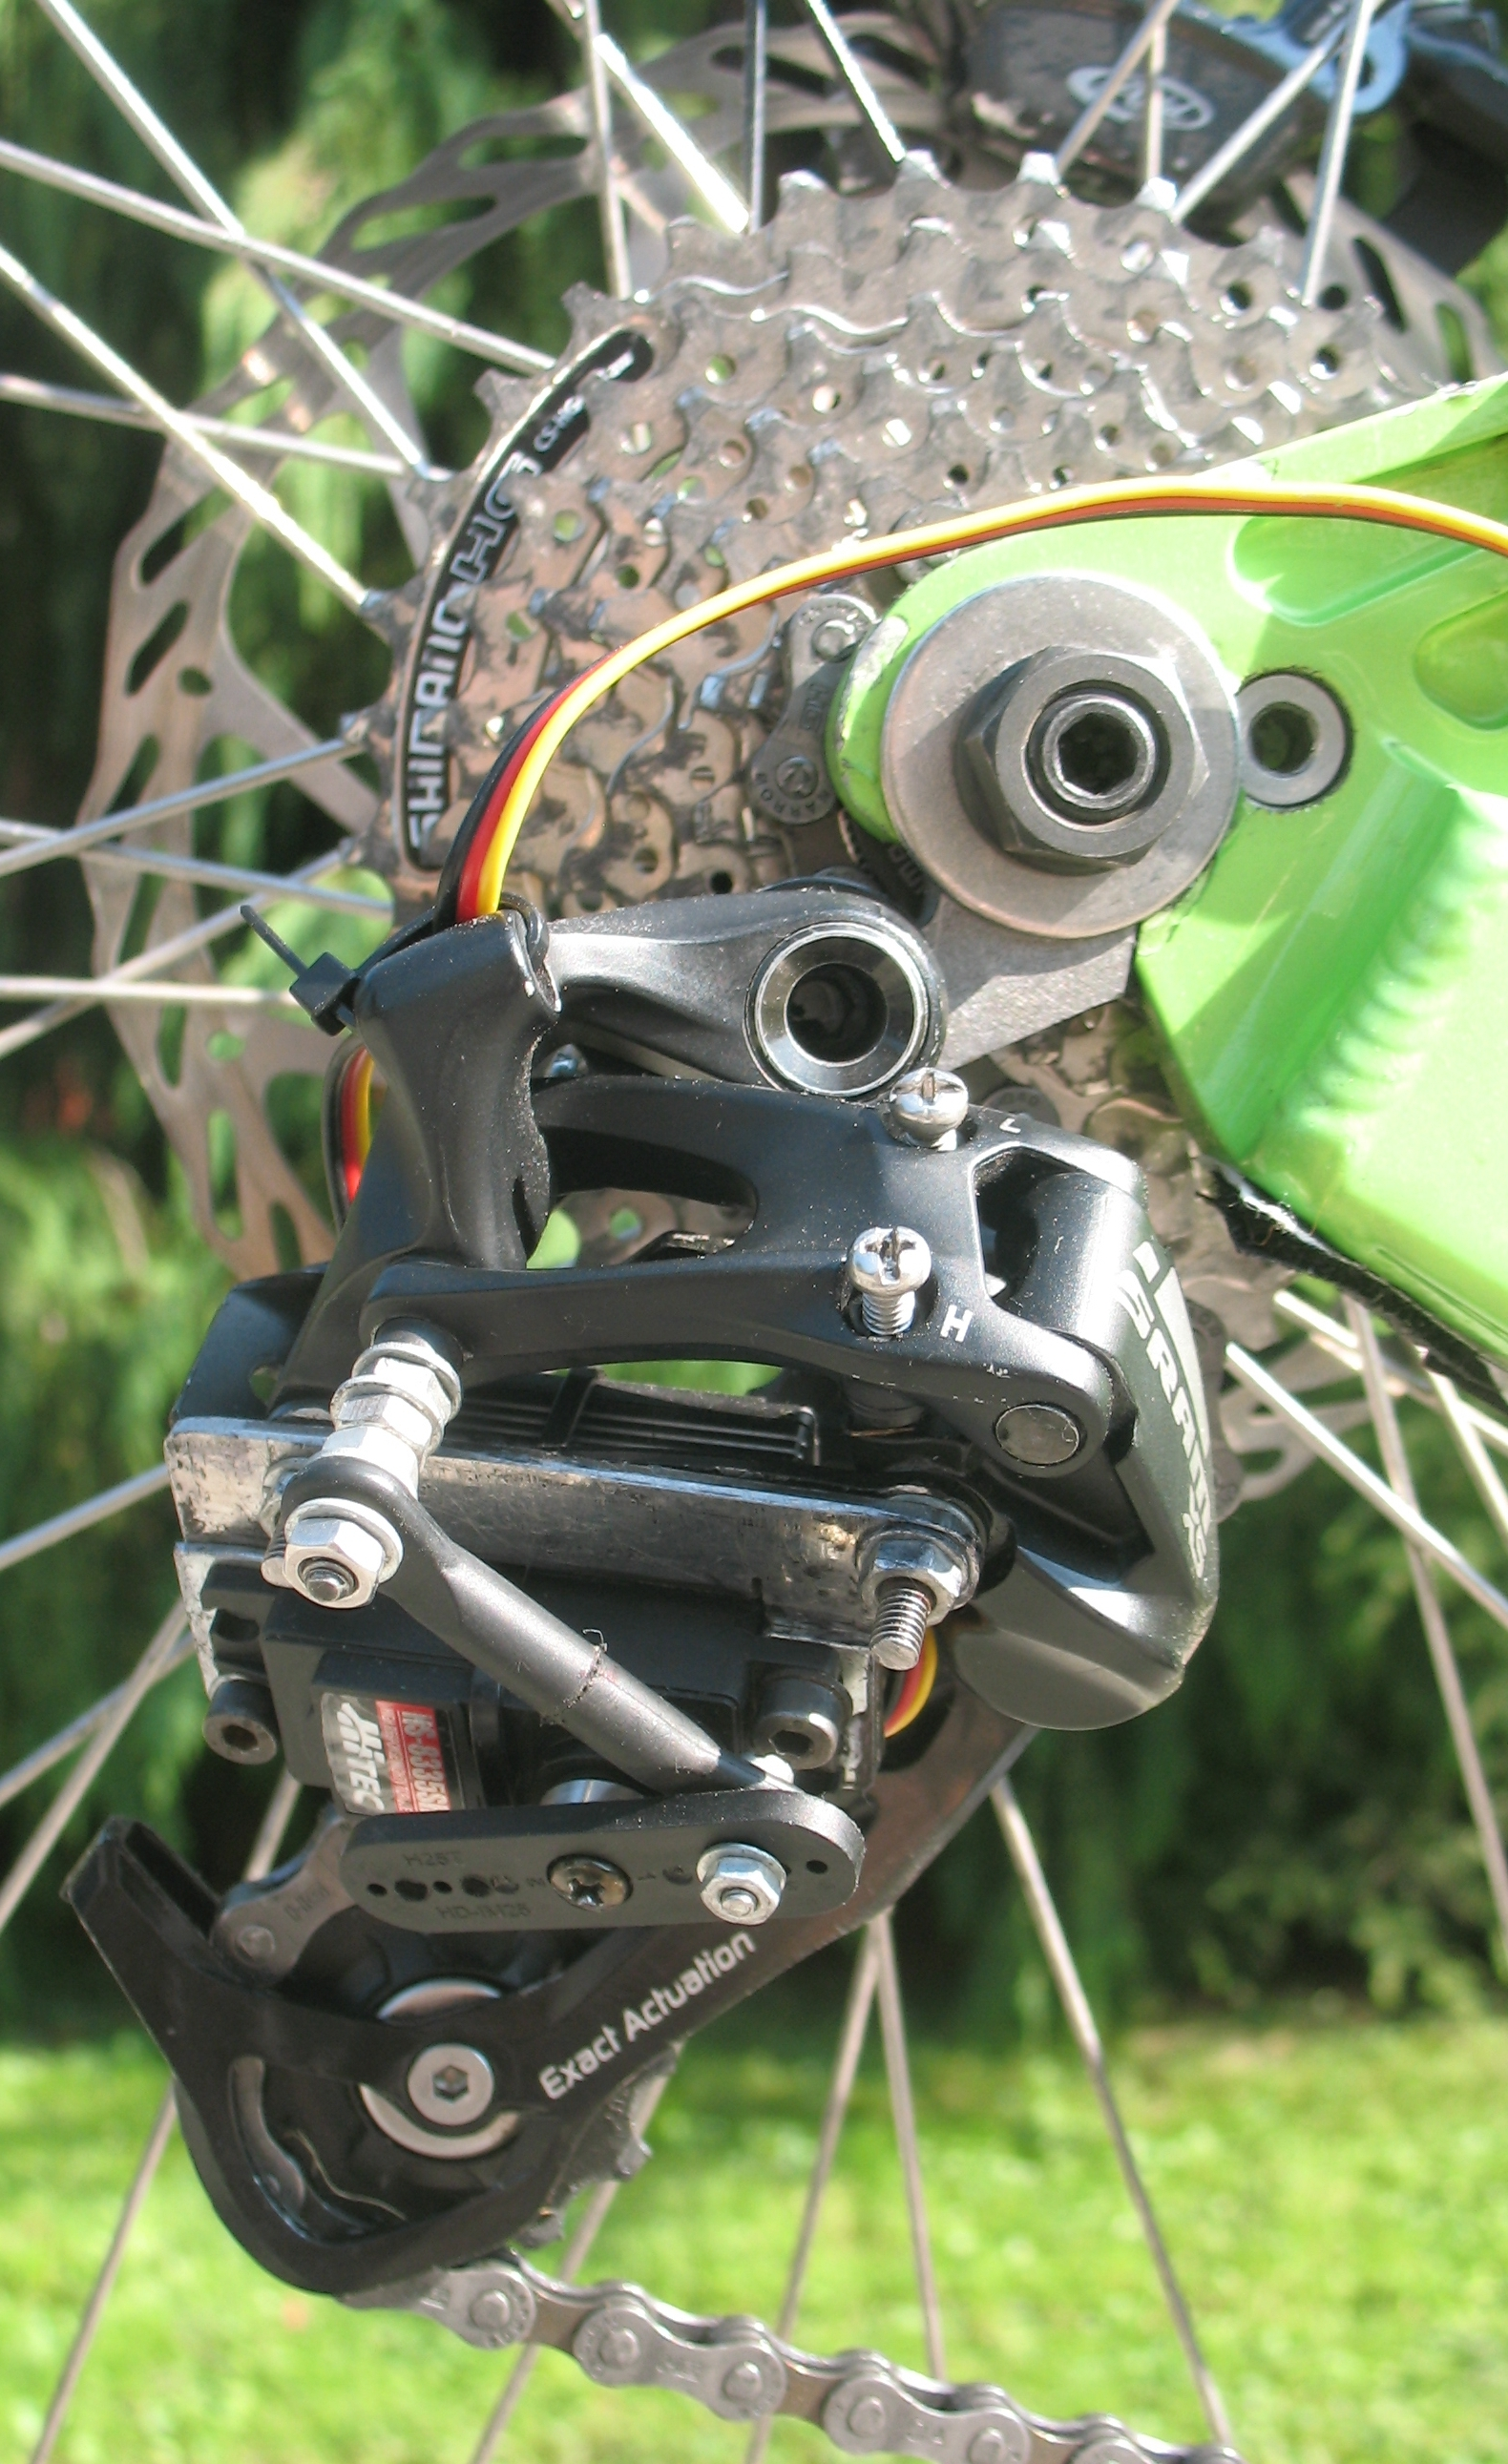
\includegraphics[scale=0.065]{przerzutka8bieg.jpg}
  \caption{Przerzutka w pozycji biegu nr 8}

\end{subfigure}
\caption{Pozycja przerzutki dla skrajnych przełożeń}
\label{fig:test}
\end{figure}

\begin{figure}[h]
\centering
\begin{subfigure}{.4\textwidth}
  \centering
  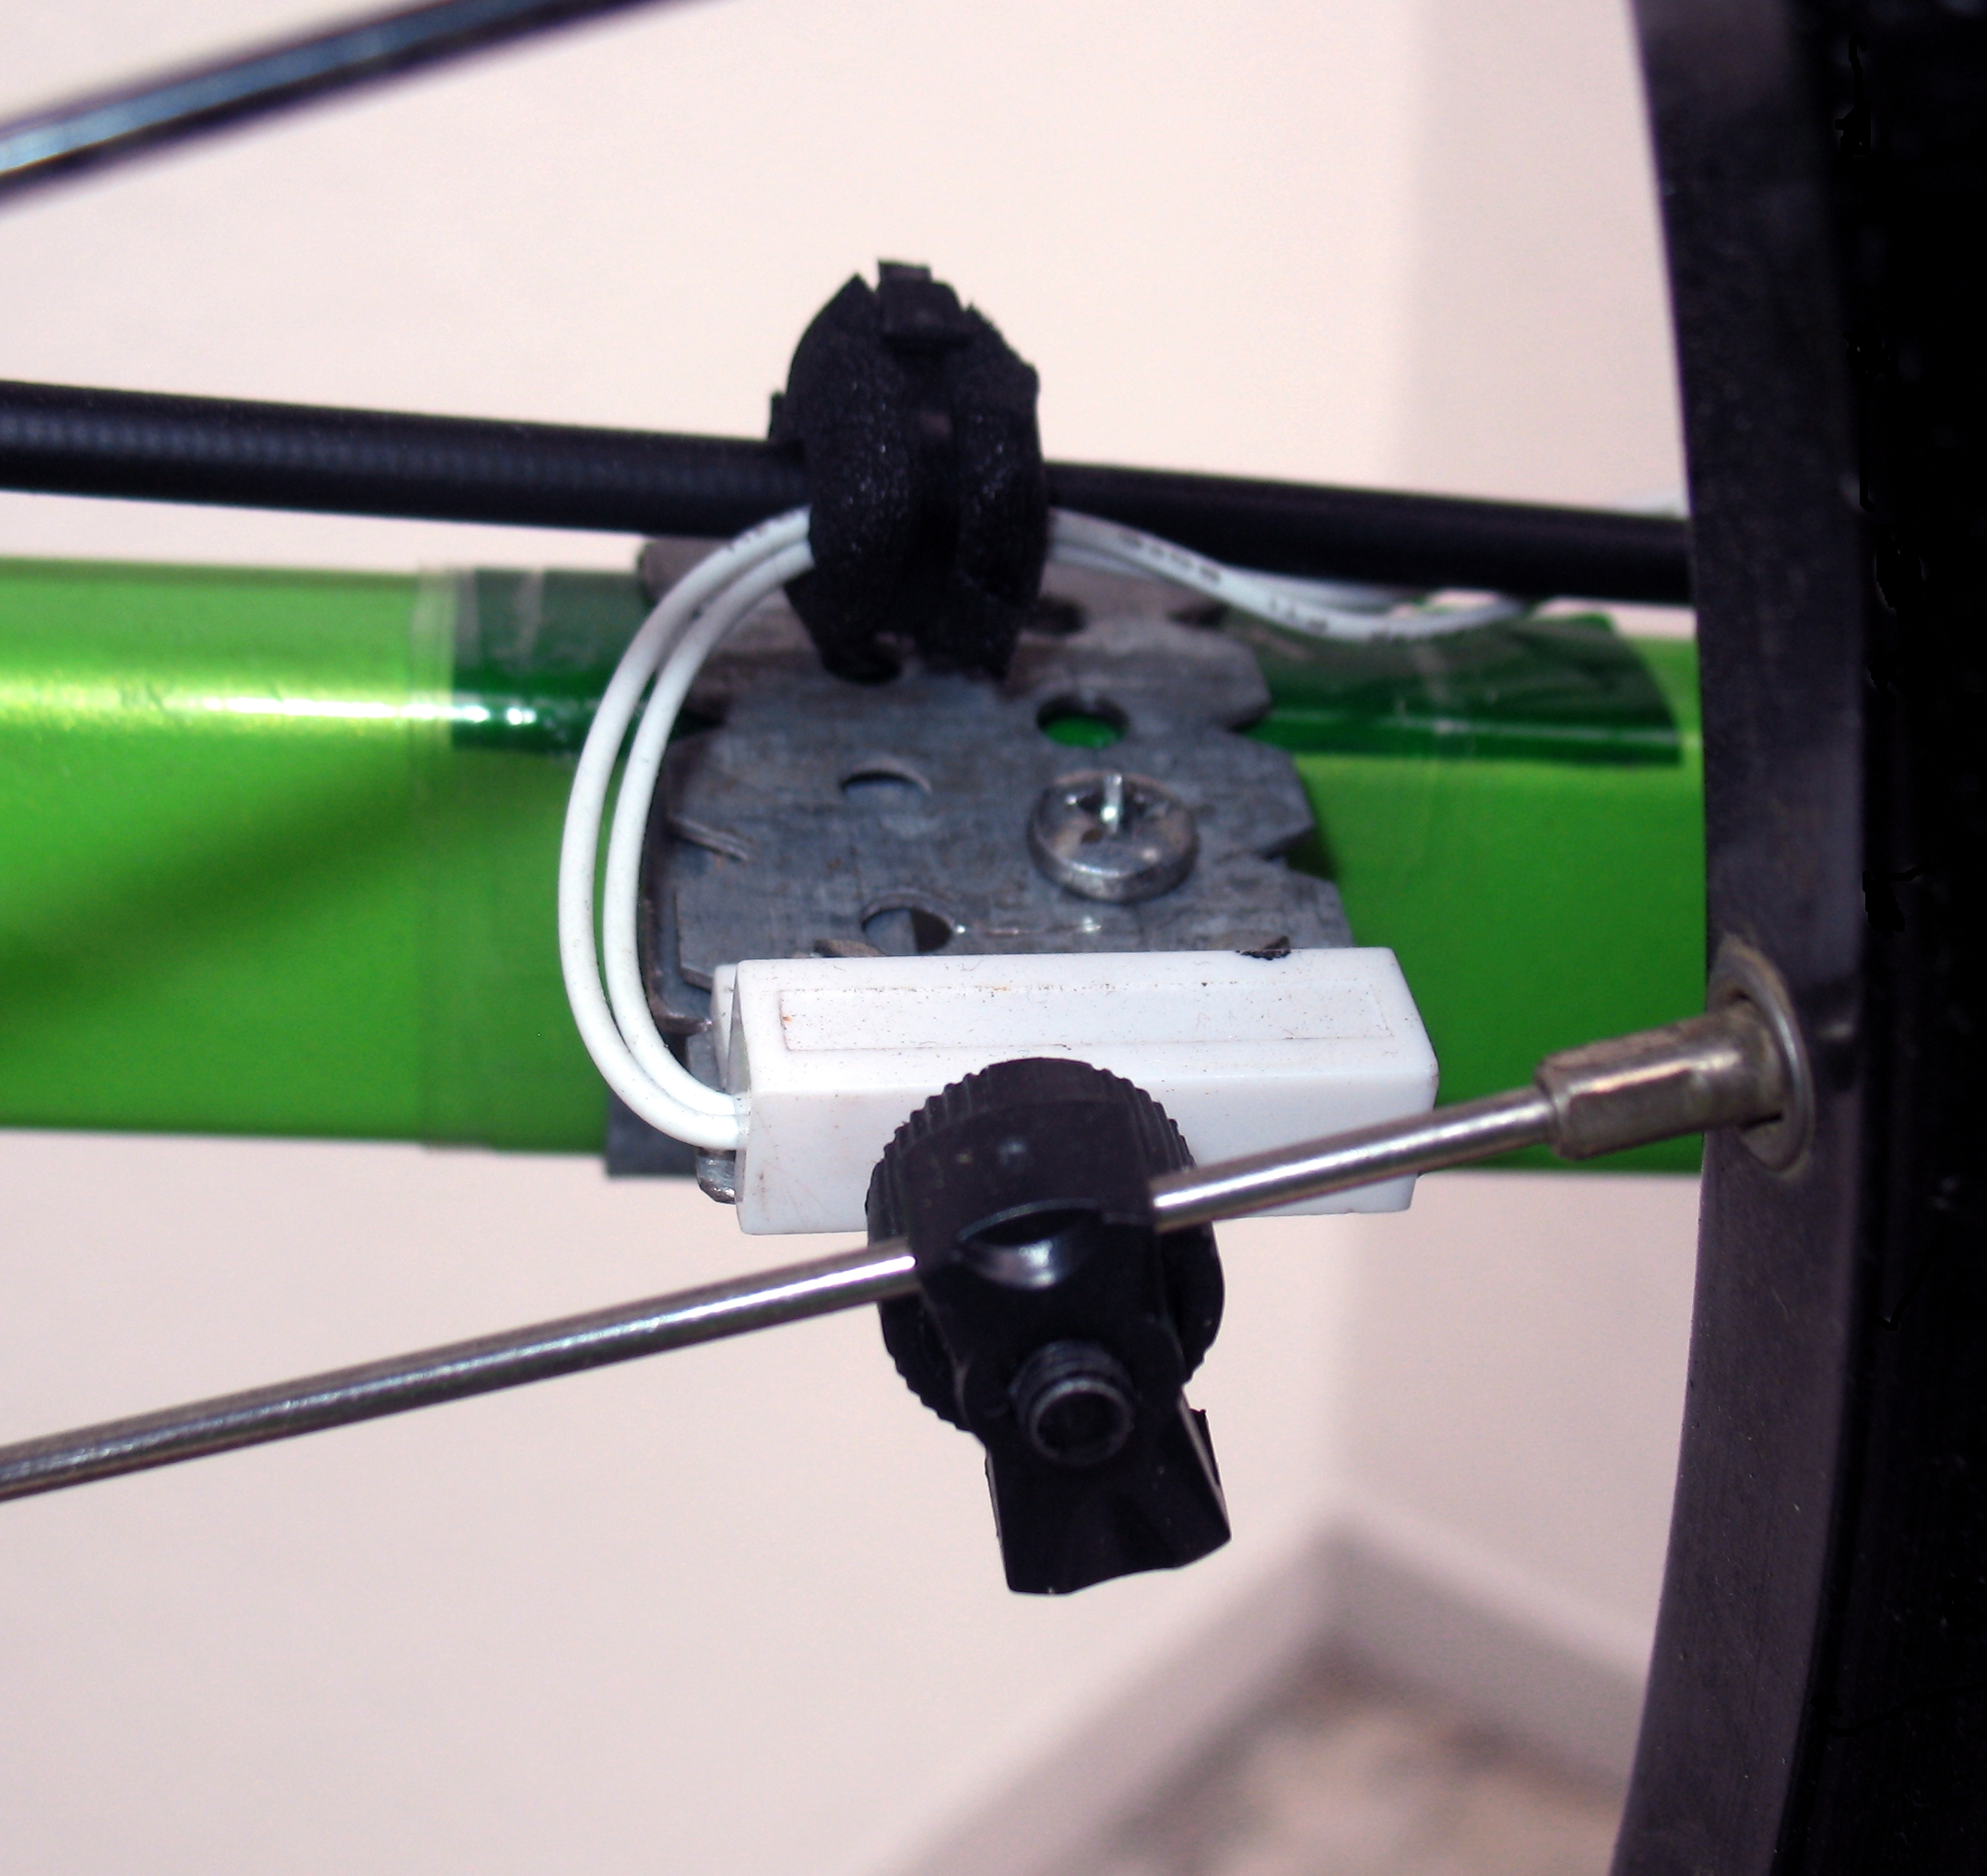
\includegraphics[scale=0.06]{przerzutkaCzujnikPredkosci.jpg}
  \caption{Czujnik prędkości roweru}
\end{subfigure}
\begin{subfigure}{.4\textwidth}
  \centering
  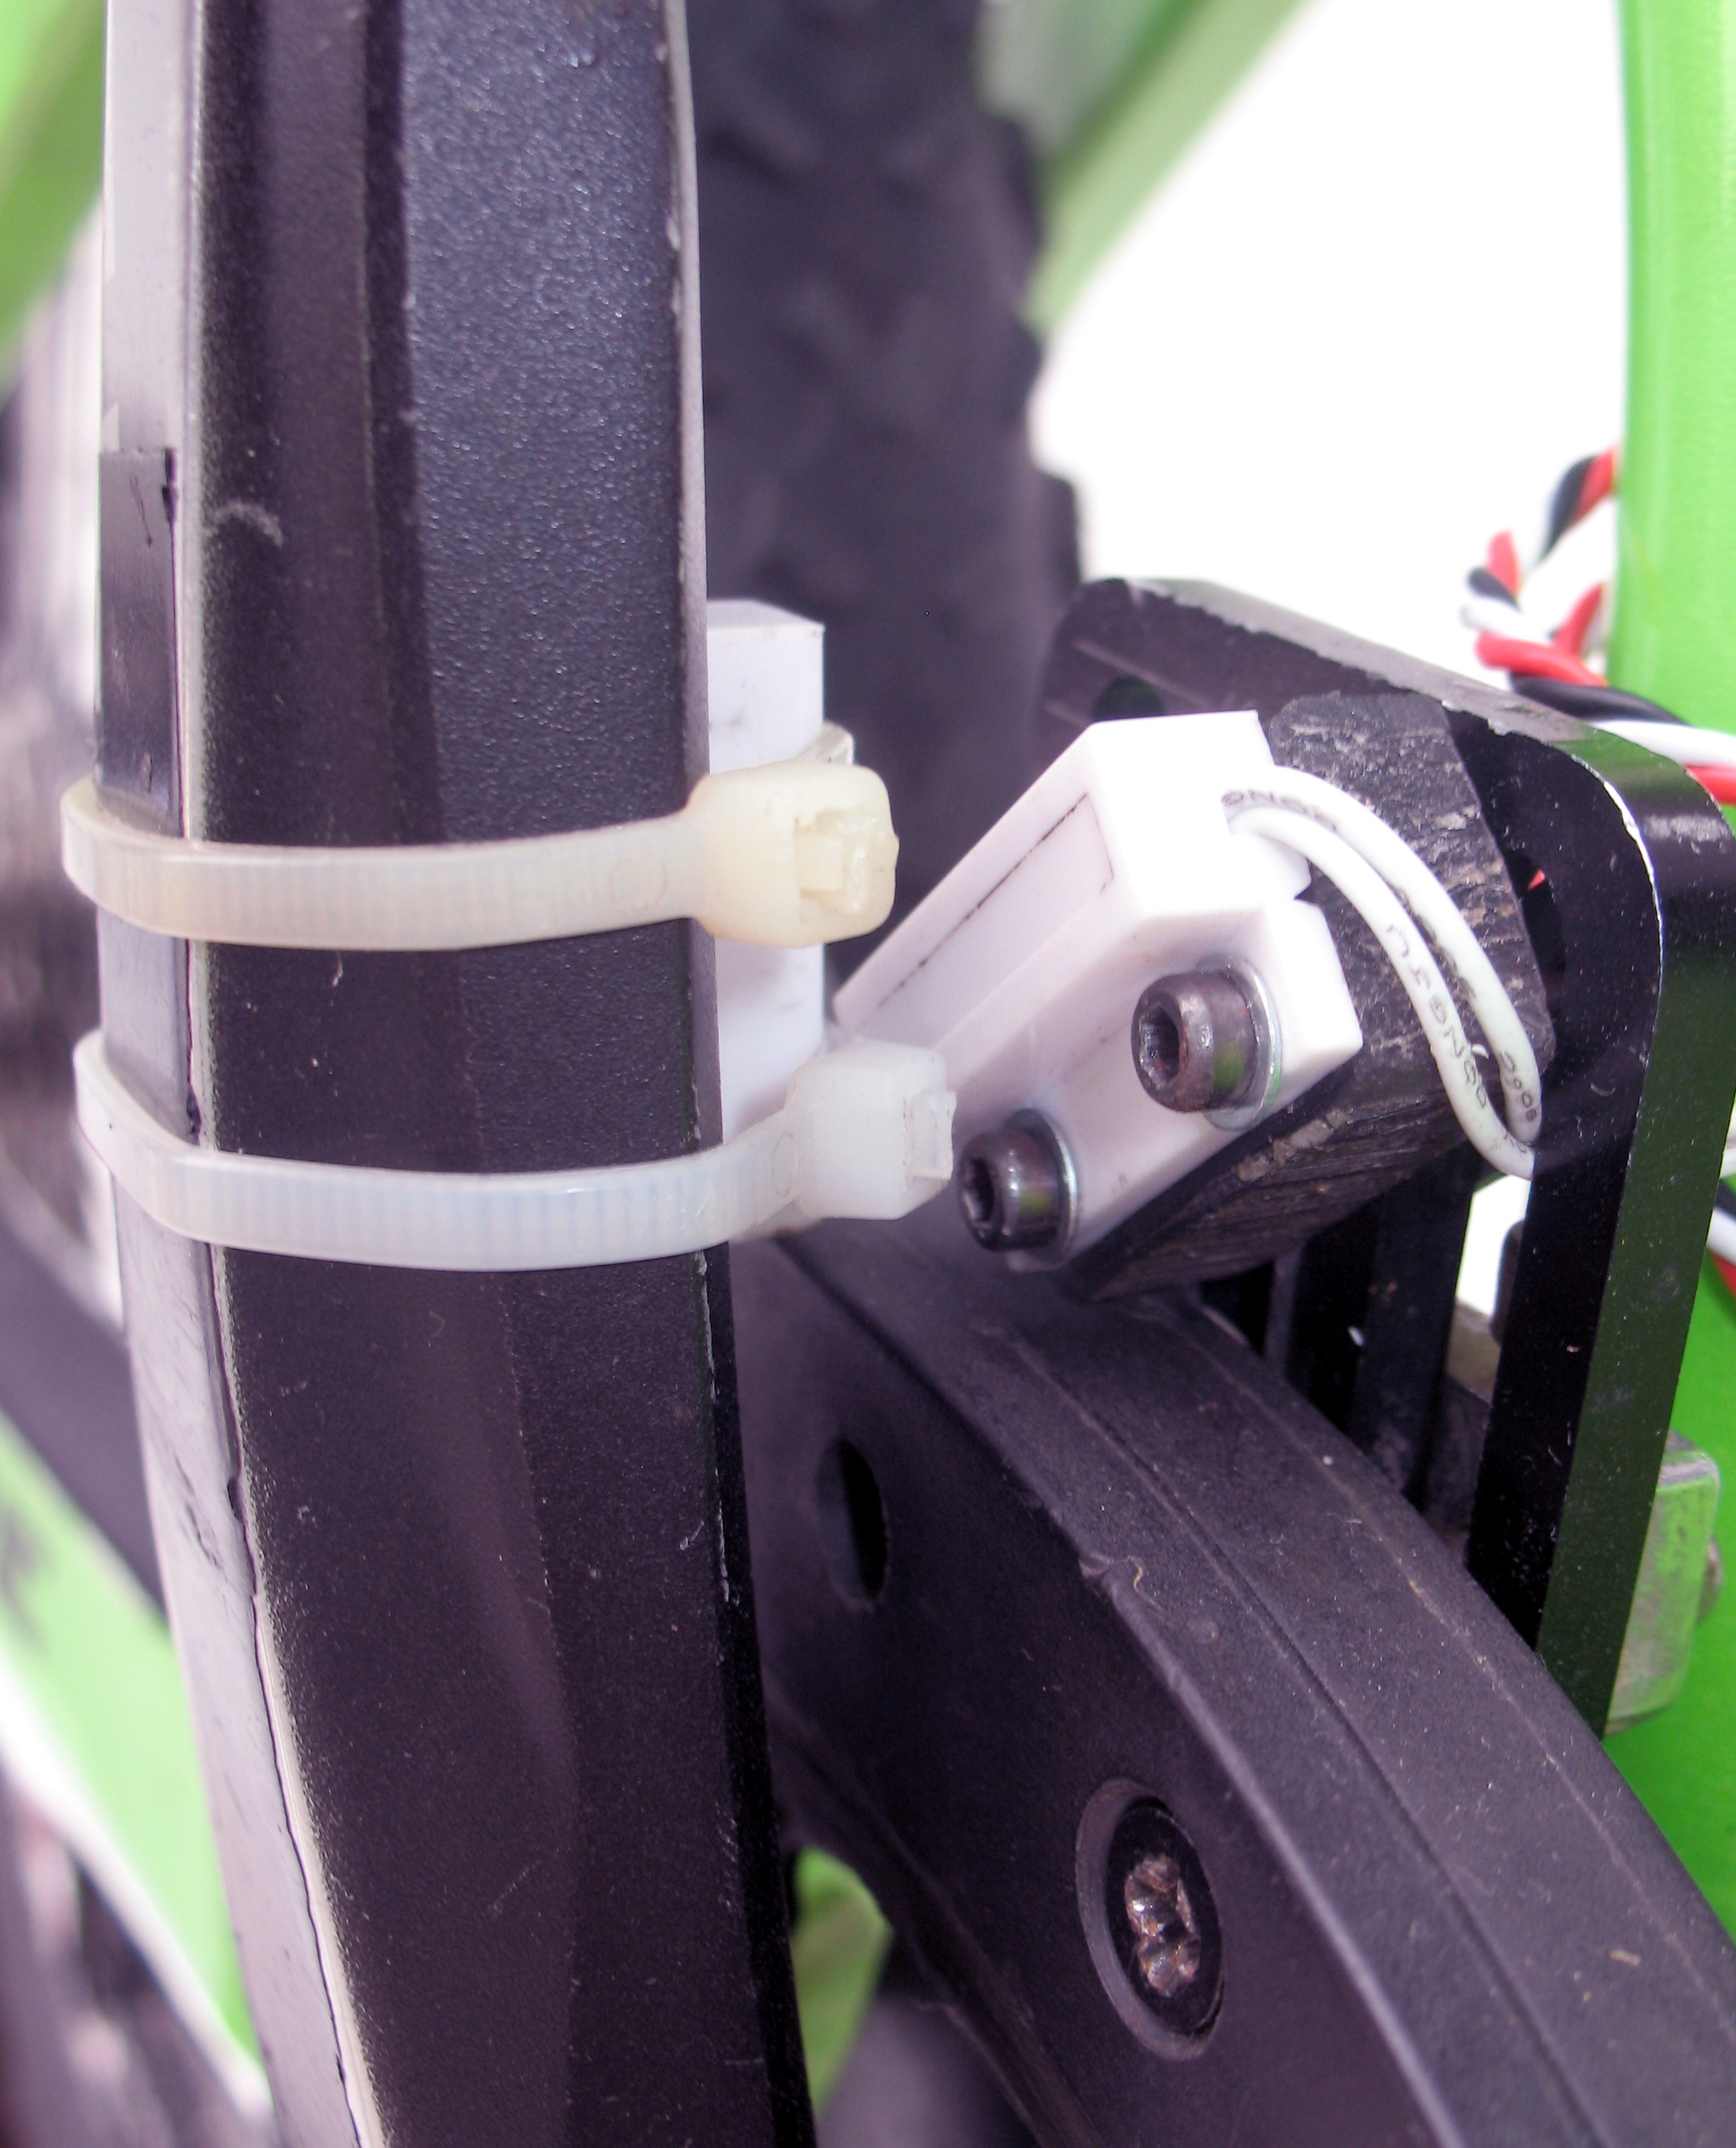
\includegraphics[scale=0.05]{przerzutkaKorba.jpg}
  \caption{Czujnik kadencji}

\end{subfigure}
\caption{Czujniki magnetyczne}
\label{fig:test}
\end{figure}

\begin{figure}[h]
\centering
\begin{subfigure}{.4\textwidth}
  \centering
  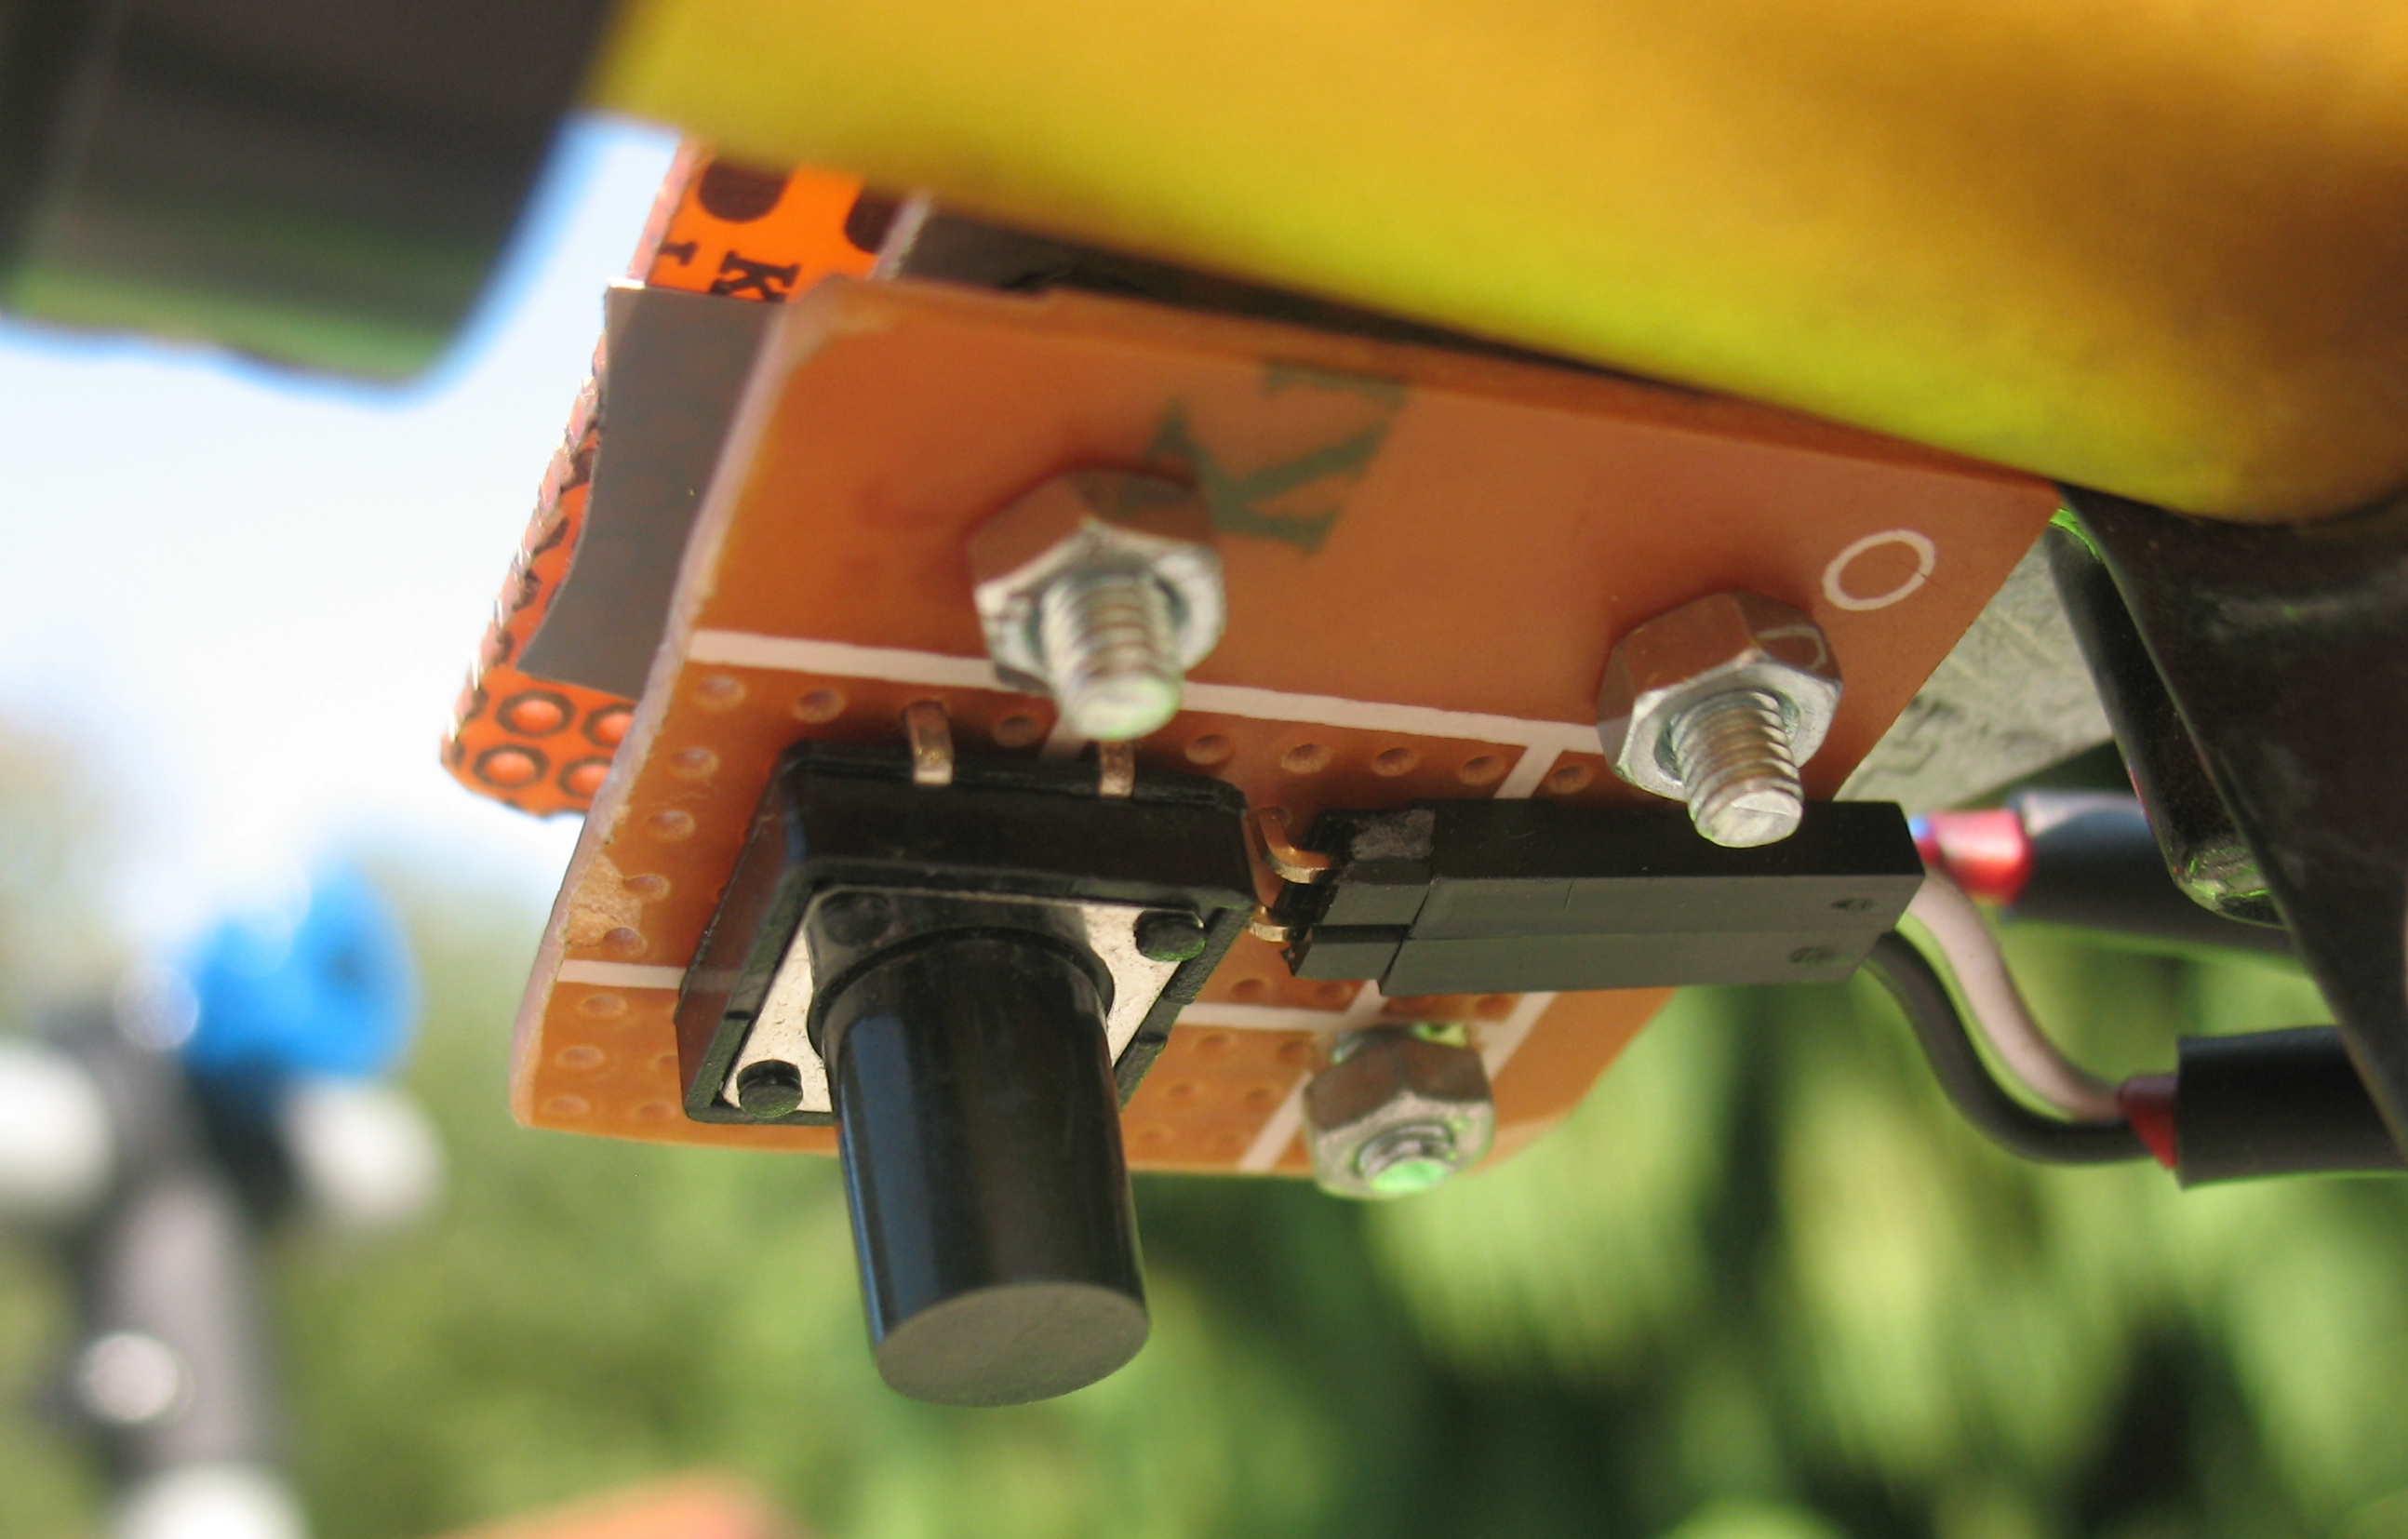
\includegraphics[scale=0.06]{manetka1.jpg}
  \caption{Przycisk redukujący bieg}
\end{subfigure}
\begin{subfigure}{.4\textwidth}
  \centering
  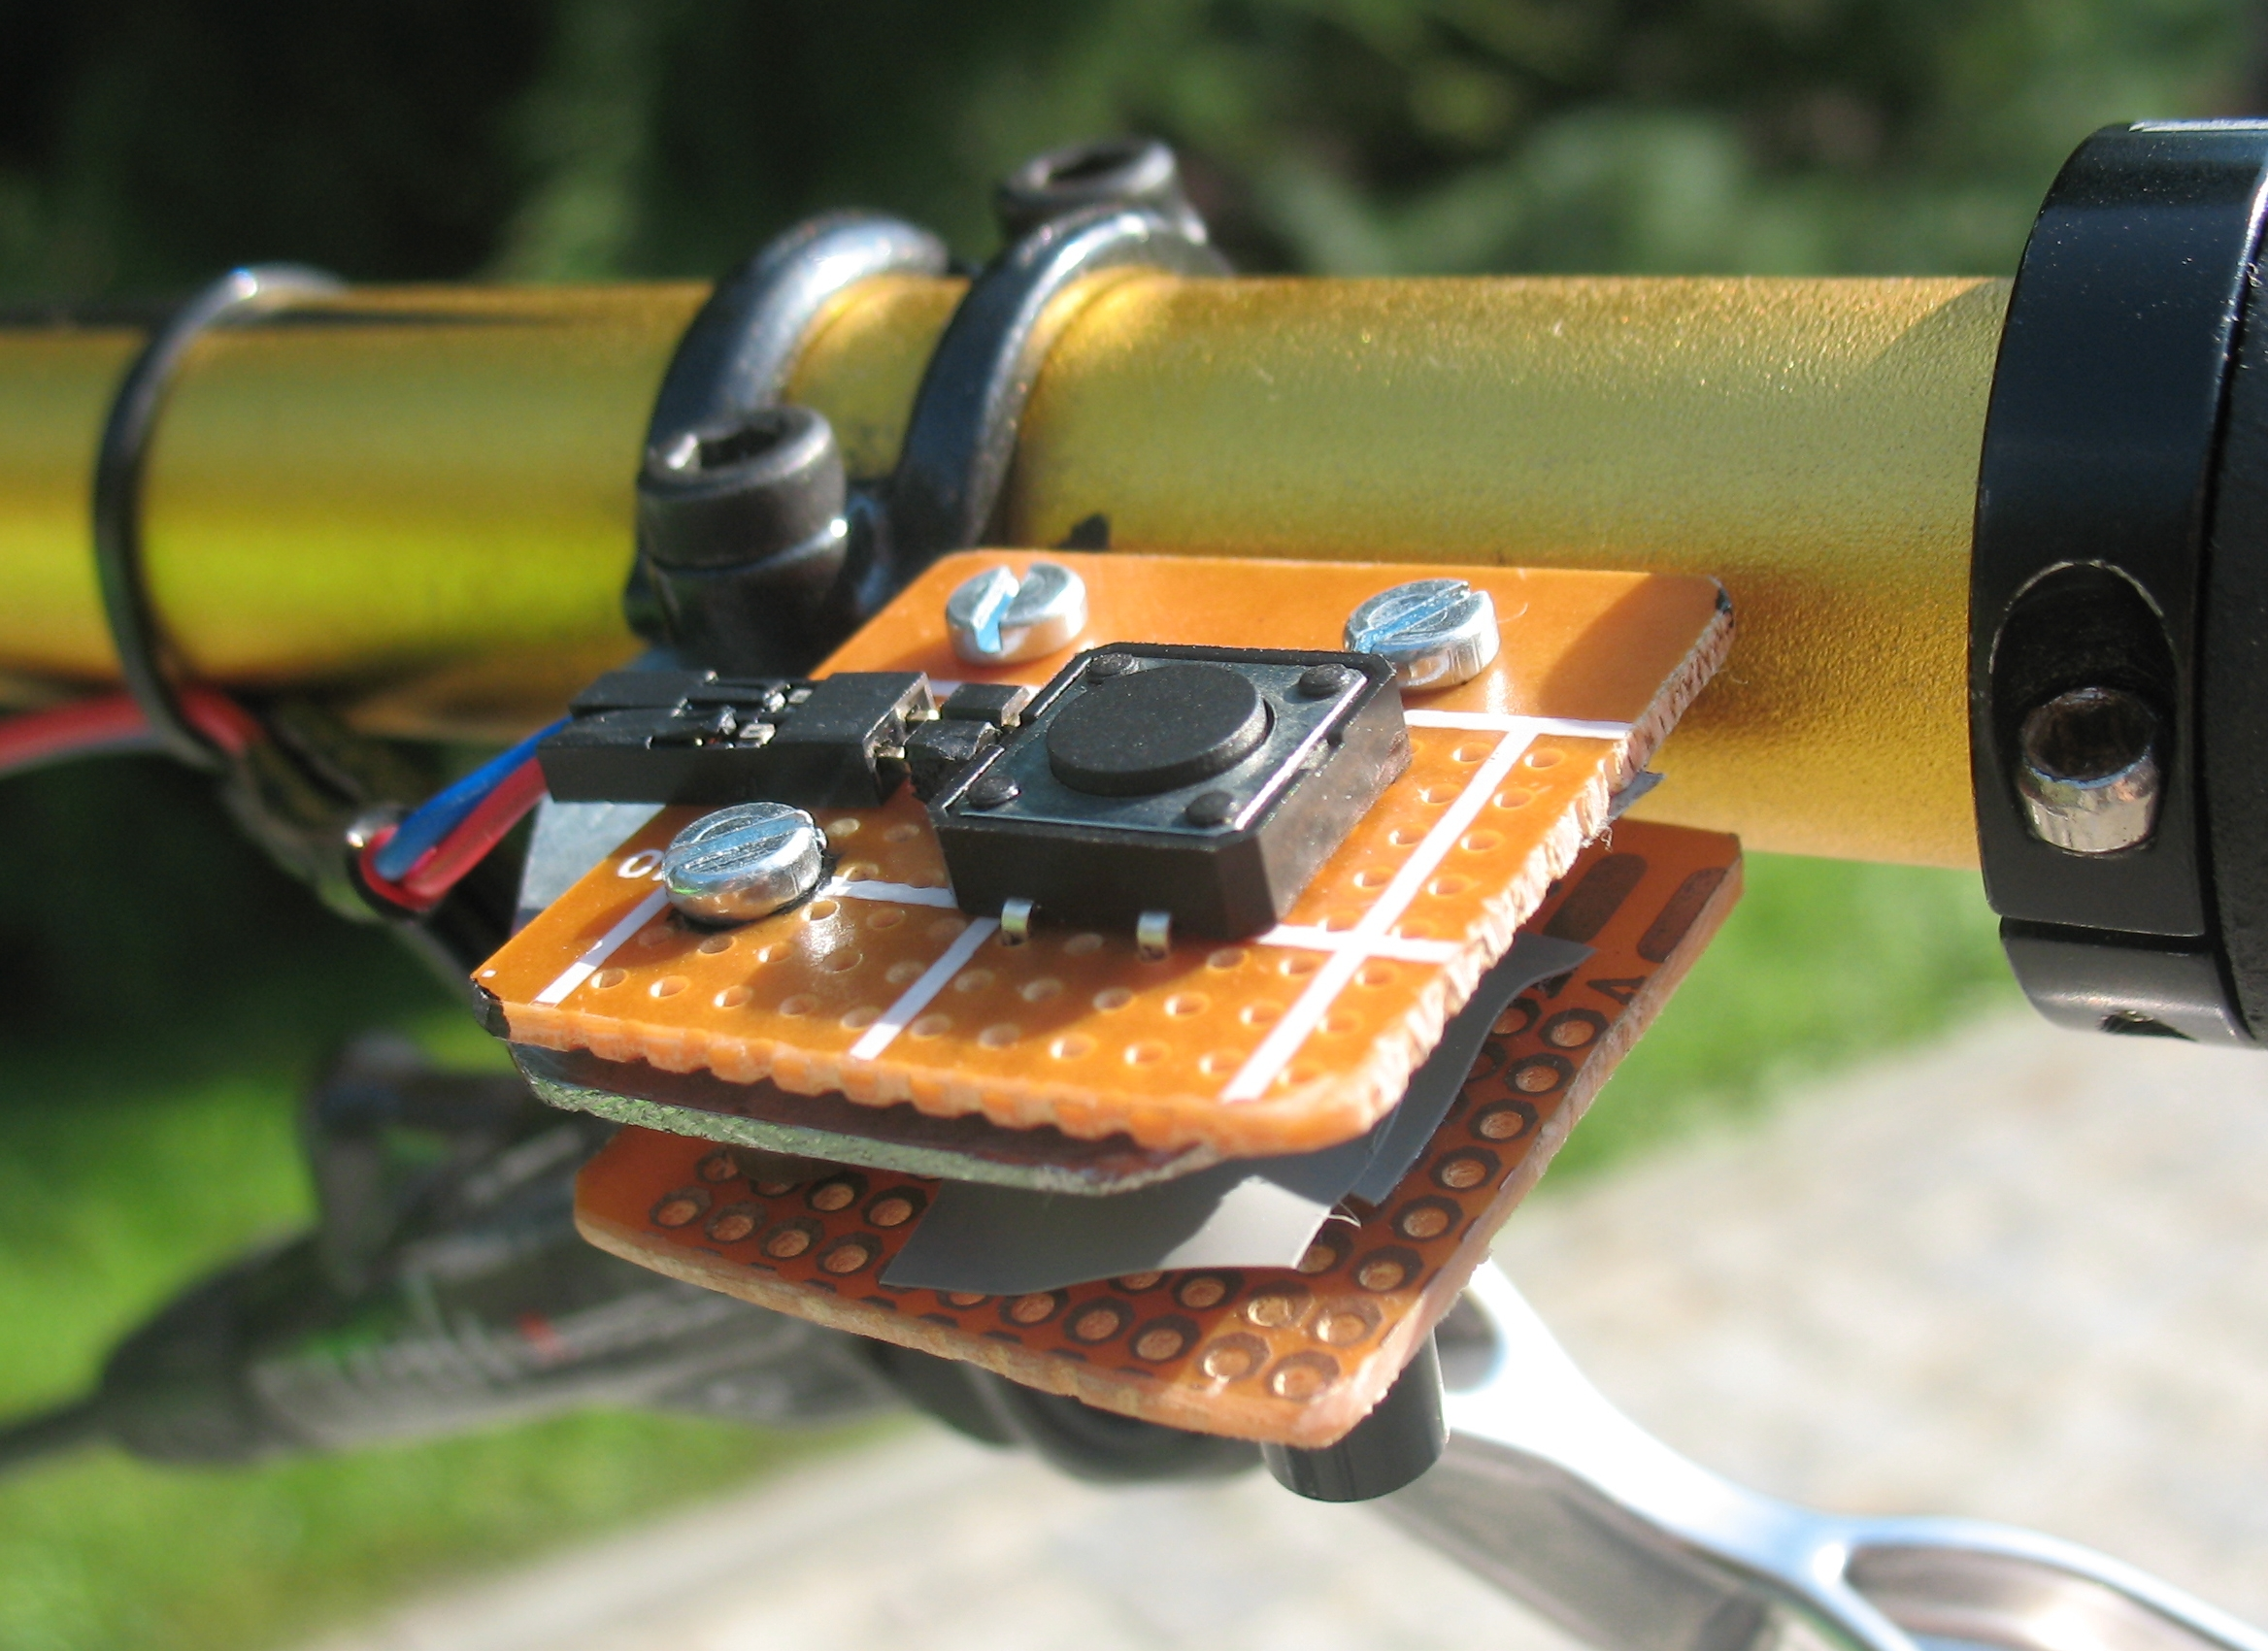
\includegraphics[scale=0.06]{manetka2.jpg}
  \caption{Przycisk zwiększający bieg}
\end{subfigure}
\caption{Manetka do zmiany przełożeń}
\label{fig:test}
\end{figure}

\begin{figure}[h]
    \centering
    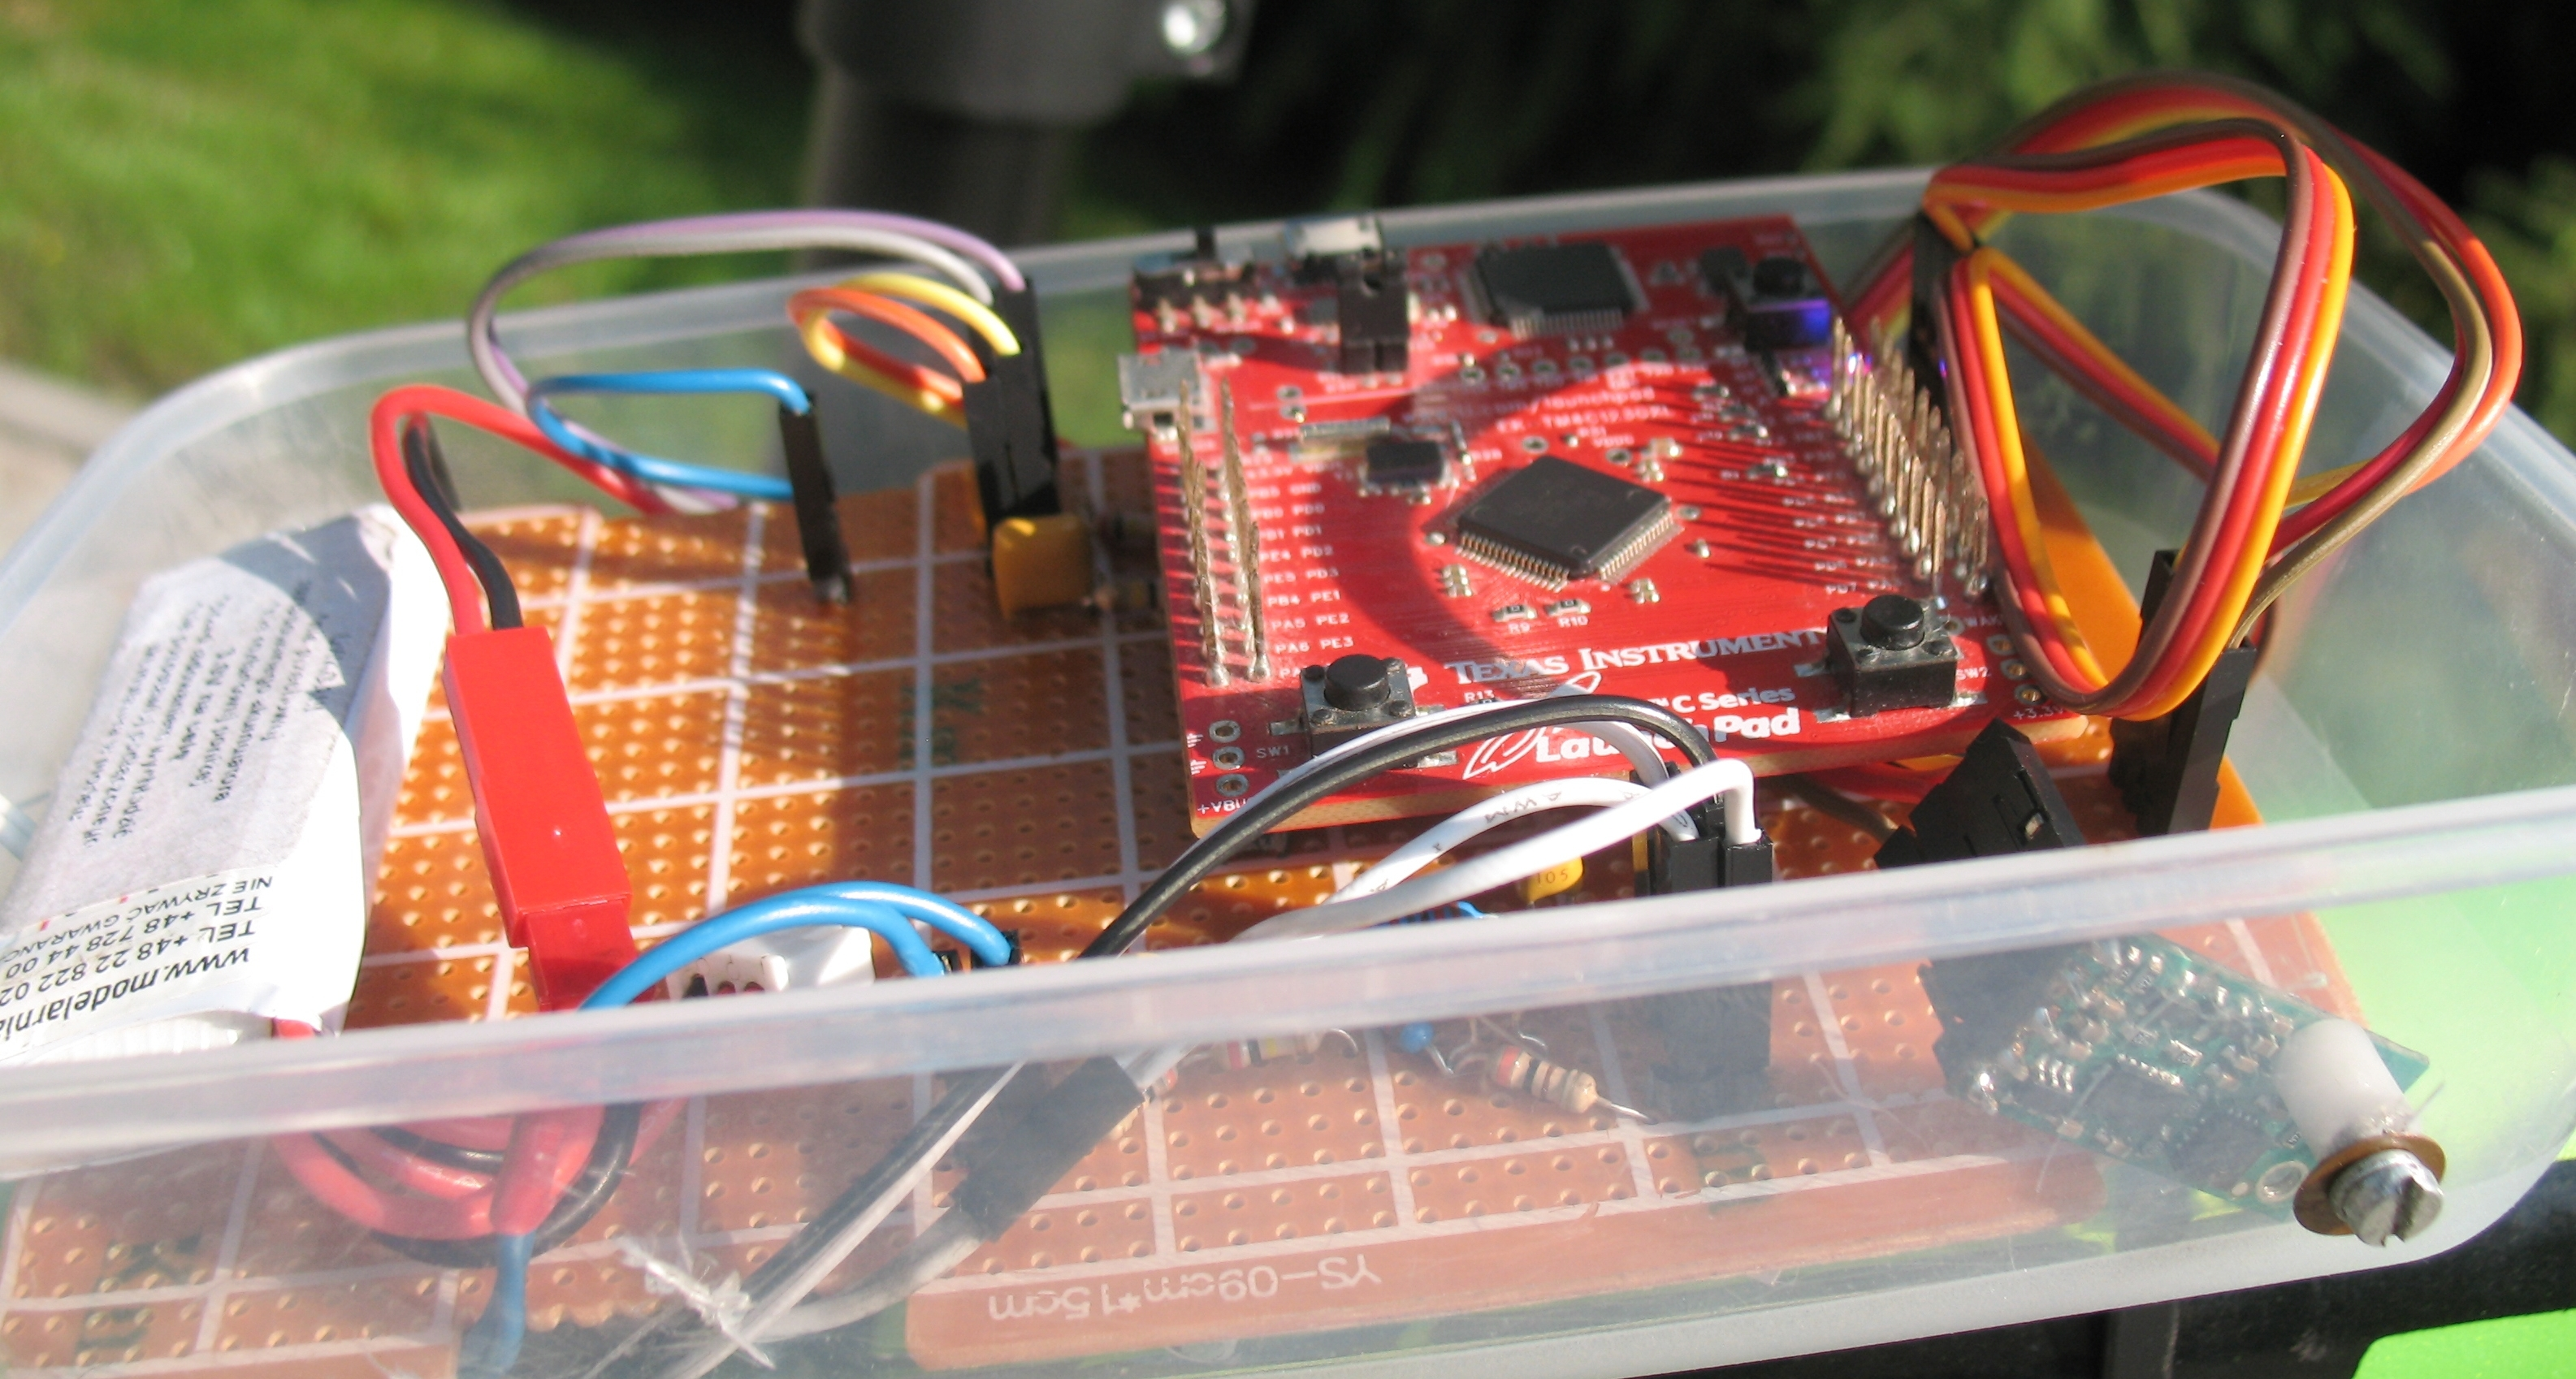
\includegraphics[scale=0.072]{przerzutkaSterownik.jpg}
    \caption{Sterownik układu}
    \label{fig:sterownik}
\end{figure}